\documentclass[twoside]{book}

% Packages required by doxygen
\usepackage{fixltx2e}
\usepackage{calc}
\usepackage{doxygen}
\usepackage[export]{adjustbox} % also loads graphicx
\usepackage{graphicx}
\usepackage[utf8]{inputenc}
\usepackage{makeidx}
\usepackage{multicol}
\usepackage{multirow}
\PassOptionsToPackage{warn}{textcomp}
\usepackage{textcomp}
\usepackage[nointegrals]{wasysym}
\usepackage[table]{xcolor}

% Font selection
\usepackage[T1]{fontenc}
\usepackage[scaled=.90]{helvet}
\usepackage{courier}
\usepackage{amssymb}
\usepackage{sectsty}
\renewcommand{\familydefault}{\sfdefault}
\allsectionsfont{%
  \fontseries{bc}\selectfont%
  \color{darkgray}%
}
\renewcommand{\DoxyLabelFont}{%
  \fontseries{bc}\selectfont%
  \color{darkgray}%
}
\newcommand{\+}{\discretionary{\mbox{\scriptsize$\hookleftarrow$}}{}{}}

% Page & text layout
\usepackage{geometry}
\geometry{%
  a4paper,%
  top=2.5cm,%
  bottom=2.5cm,%
  left=2.5cm,%
  right=2.5cm%
}
\tolerance=750
\hfuzz=15pt
\hbadness=750
\setlength{\emergencystretch}{15pt}
\setlength{\parindent}{0cm}
\setlength{\parskip}{3ex plus 2ex minus 2ex}
\makeatletter
\renewcommand{\paragraph}{%
  \@startsection{paragraph}{4}{0ex}{-1.0ex}{1.0ex}{%
    \normalfont\normalsize\bfseries\SS@parafont%
  }%
}
\renewcommand{\subparagraph}{%
  \@startsection{subparagraph}{5}{0ex}{-1.0ex}{1.0ex}{%
    \normalfont\normalsize\bfseries\SS@subparafont%
  }%
}
\makeatother

% Headers & footers
\usepackage{fancyhdr}
\pagestyle{fancyplain}
\fancyhead[LE]{\fancyplain{}{\bfseries\thepage}}
\fancyhead[CE]{\fancyplain{}{}}
\fancyhead[RE]{\fancyplain{}{\bfseries\leftmark}}
\fancyhead[LO]{\fancyplain{}{\bfseries\rightmark}}
\fancyhead[CO]{\fancyplain{}{}}
\fancyhead[RO]{\fancyplain{}{\bfseries\thepage}}
\fancyfoot[LE]{\fancyplain{}{}}
\fancyfoot[CE]{\fancyplain{}{}}
\fancyfoot[RE]{\fancyplain{}{\bfseries\scriptsize Generated by Doxygen }}
\fancyfoot[LO]{\fancyplain{}{\bfseries\scriptsize Generated by Doxygen }}
\fancyfoot[CO]{\fancyplain{}{}}
\fancyfoot[RO]{\fancyplain{}{}}
\renewcommand{\footrulewidth}{0.4pt}
\renewcommand{\chaptermark}[1]{%
  \markboth{#1}{}%
}
\renewcommand{\sectionmark}[1]{%
  \markright{\thesection\ #1}%
}

% Indices & bibliography
\usepackage{natbib}
\usepackage[titles]{tocloft}
\setcounter{tocdepth}{3}
\setcounter{secnumdepth}{5}
\makeindex

% Custom commands
\newcommand{\clearemptydoublepage}{%
  \newpage{\pagestyle{empty}\cleardoublepage}%
}

\usepackage{caption}
\captionsetup{labelsep=space,justification=centering,font={bf},singlelinecheck=off,skip=4pt,position=top}

%===== C O N T E N T S =====

\begin{document}

% Titlepage & ToC
\pagenumbering{roman}
\begin{titlepage}
\vspace*{7cm}
\begin{center}%
{\Large T\+P1 }\\
\vspace*{1cm}
{\large Generated by Doxygen 1.8.11}\\
\end{center}
\end{titlepage}
\clearemptydoublepage
\tableofcontents
\clearemptydoublepage
\pagenumbering{arabic}

%--- Begin generated contents ---
\chapter{Data Structure Index}
\section{Data Structures}
Here are the data structures with brief descriptions\+:\begin{DoxyCompactList}
\item\contentsline{section}{\textbf{ Login} }{\pageref{struct_login}}{}
\end{DoxyCompactList}

\chapter{File Index}
\section{File List}
Here is a list of all files with brief descriptions\+:\begin{DoxyCompactList}
\item\contentsline{section}{/home/torce/\+Desktop/\+Juan\+Soriano/\+T\+P1/src/baash/{\bf archfunc.\+c} }{\pageref{archfunc_8c}}{}
\item\contentsline{section}{/home/torce/\+Desktop/\+Juan\+Soriano/\+T\+P1/src/baash/{\bf archfunc.\+h} }{\pageref{archfunc_8h}}{}
\item\contentsline{section}{/home/torce/\+Desktop/\+Juan\+Soriano/\+T\+P1/src/baash/{\bf evalfunc.\+c} }{\pageref{evalfunc_8c}}{}
\item\contentsline{section}{/home/torce/\+Desktop/\+Juan\+Soriano/\+T\+P1/src/baash/{\bf evalfunc.\+h} }{\pageref{evalfunc_8h}}{}
\item\contentsline{section}{/home/torce/\+Desktop/\+Juan\+Soriano/\+T\+P1/src/baash/{\bf main.\+c} }{\pageref{baash_2main_8c}}{}
\item\contentsline{section}{/home/torce/\+Desktop/\+Juan\+Soriano/\+T\+P1/src/client/{\bf main.\+c} }{\pageref{client_2main_8c}}{}
\item\contentsline{section}{/home/torce/\+Desktop/\+Juan\+Soriano/\+T\+P1/src/server/{\bf main.\+c} }{\pageref{server_2main_8c}}{}
\end{DoxyCompactList}

\chapter{Data Structure Documentation}
\section{Login Struct Reference}
\label{struct_login}\index{Login@{Login}}
\subsection*{Data Fields}
\begin{DoxyCompactItemize}
\item 
char \textbf{ name} [\textbf{ S\+N\+A\+ME}]
\item 
char \textbf{ password} [\textbf{ S\+N\+A\+ME}]
\end{DoxyCompactItemize}


\subsection{Field Documentation}
\mbox{\label{struct_login_a9e46adf32ce202b0f33097479dce0f74}} 
\index{Login@{Login}!name@{name}}
\index{name@{name}!Login@{Login}}
\subsubsection{name}
{\footnotesize\ttfamily char name[\textbf{ S\+N\+A\+ME}]}

\mbox{\label{struct_login_ac7b9e627171bb0d214aea70b4ca9d5c6}} 
\index{Login@{Login}!password@{password}}
\index{password@{password}!Login@{Login}}
\subsubsection{password}
{\footnotesize\ttfamily char password[\textbf{ S\+N\+A\+ME}]}



The documentation for this struct was generated from the following file\+:\begin{DoxyCompactItemize}
\item 
/home/torce/\+Facultad/\+S\+O2/so2/\+T\+P1/src/server/\textbf{ main.\+c}\end{DoxyCompactItemize}

\section{sockbuff Struct Reference}
\label{structsockbuff}\index{sockbuff@{sockbuff}}
\subsection*{Data Fields}
\begin{DoxyCompactItemize}
\item 
int {\bf sockfd}
\item 
char $\ast$ {\bf buffer}
\item 
size\+\_\+t {\bf buffer\+\_\+size}
\end{DoxyCompactItemize}


\subsection{Field Documentation}
\index{sockbuff@{sockbuff}!buffer@{buffer}}
\index{buffer@{buffer}!sockbuff@{sockbuff}}
\subsubsection[{buffer}]{\setlength{\rightskip}{0pt plus 5cm}char$\ast$ buffer}\label{structsockbuff_aff2566f4c366b48d73479bef43ee4d2e}
\index{sockbuff@{sockbuff}!buffer\+\_\+size@{buffer\+\_\+size}}
\index{buffer\+\_\+size@{buffer\+\_\+size}!sockbuff@{sockbuff}}
\subsubsection[{buffer\+\_\+size}]{\setlength{\rightskip}{0pt plus 5cm}size\+\_\+t buffer\+\_\+size}\label{structsockbuff_a799a743b3abd553a37fc01ad3097df08}
\index{sockbuff@{sockbuff}!sockfd@{sockfd}}
\index{sockfd@{sockfd}!sockbuff@{sockbuff}}
\subsubsection[{sockfd}]{\setlength{\rightskip}{0pt plus 5cm}int sockfd}\label{structsockbuff_ad2c8fb3df3a737e0685e902870a611d2}


The documentation for this struct was generated from the following file\+:\begin{DoxyCompactItemize}
\item 
/home/torce/\+Desktop/\+Juan\+Soriano/\+T\+P1/src/client/{\bf main.\+c}\end{DoxyCompactItemize}

\chapter{File Documentation}
\section{/home/torce/\+Desktop/\+Juan\+Soriano/\+T\+P1/src/baash/archfunc.c File Reference}
\label{archfunc_8c}\index{/home/torce/\+Desktop/\+Juan\+Soriano/\+T\+P1/src/baash/archfunc.\+c@{/home/torce/\+Desktop/\+Juan\+Soriano/\+T\+P1/src/baash/archfunc.\+c}}
{\ttfamily \#include $<$stdio.\+h$>$}\\*
{\ttfamily \#include $<$stdlib.\+h$>$}\\*
{\ttfamily \#include $<$unistd.\+h$>$}\\*
{\ttfamily \#include $<$string.\+h$>$}\\*
{\ttfamily \#include $<$fcntl.\+h$>$}\\*
{\ttfamily \#include \char`\"{}archfunc.\+h\char`\"{}}\\*
Include dependency graph for archfunc.\+c\+:
\nopagebreak
\begin{figure}[H]
\begin{center}
\leavevmode
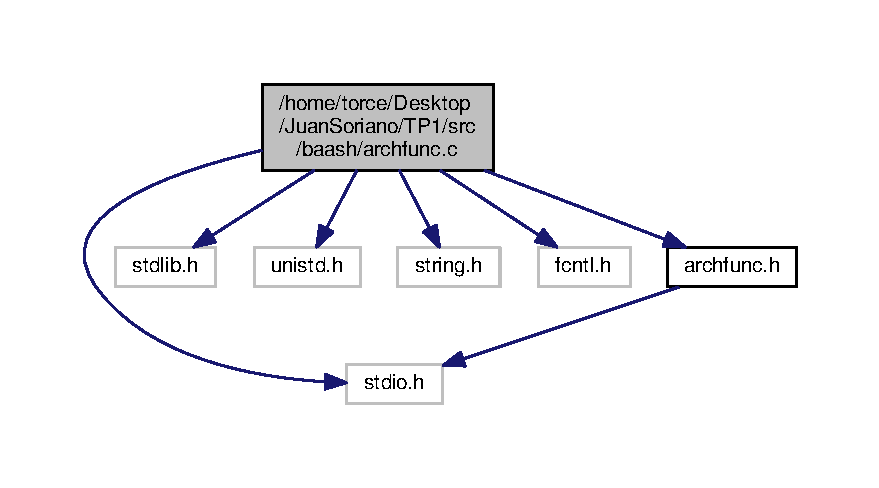
\includegraphics[width=350pt]{archfunc_8c__incl}
\end{center}
\end{figure}
\subsection*{Functions}
\begin{DoxyCompactItemize}
\item 
void {\bf buscar\+Archivo} (char $\ast$file, char $\ast$$\ast$carpetas, char $\ast$command\+File)
\item 
void {\bf a\+Archivo} (char $\ast$archivo)
\item 
void {\bf de\+Archivo} (char filename[$\,$])
\end{DoxyCompactItemize}


\subsection{Function Documentation}
\index{archfunc.\+c@{archfunc.\+c}!a\+Archivo@{a\+Archivo}}
\index{a\+Archivo@{a\+Archivo}!archfunc.\+c@{archfunc.\+c}}
\subsubsection[{a\+Archivo(char $\ast$archivo)}]{\setlength{\rightskip}{0pt plus 5cm}void a\+Archivo (
\begin{DoxyParamCaption}
\item[{char $\ast$}]{archivo}
\end{DoxyParamCaption}
)}\label{archfunc_8c_a1716ae9bb2a53e7f0a27edd9b5ef6b80}
\index{archfunc.\+c@{archfunc.\+c}!buscar\+Archivo@{buscar\+Archivo}}
\index{buscar\+Archivo@{buscar\+Archivo}!archfunc.\+c@{archfunc.\+c}}
\subsubsection[{buscar\+Archivo(char $\ast$file, char $\ast$$\ast$carpetas, char $\ast$command\+File)}]{\setlength{\rightskip}{0pt plus 5cm}void buscar\+Archivo (
\begin{DoxyParamCaption}
\item[{char $\ast$}]{file, }
\item[{char $\ast$$\ast$}]{carpetas, }
\item[{char $\ast$}]{command\+File}
\end{DoxyParamCaption}
)}\label{archfunc_8c_a39bd412666731022a74482418298eab9}
\index{archfunc.\+c@{archfunc.\+c}!de\+Archivo@{de\+Archivo}}
\index{de\+Archivo@{de\+Archivo}!archfunc.\+c@{archfunc.\+c}}
\subsubsection[{de\+Archivo(char filename[])}]{\setlength{\rightskip}{0pt plus 5cm}void de\+Archivo (
\begin{DoxyParamCaption}
\item[{char}]{filename[$\,$]}
\end{DoxyParamCaption}
)}\label{archfunc_8c_abd4ff40c4d09e464acdf313a1be515c5}

\section{/home/torce/\+Desktop/\+Juan\+Soriano/\+T\+P1/src/baash/archfunc.h File Reference}
\label{archfunc_8h}\index{/home/torce/\+Desktop/\+Juan\+Soriano/\+T\+P1/src/baash/archfunc.\+h@{/home/torce/\+Desktop/\+Juan\+Soriano/\+T\+P1/src/baash/archfunc.\+h}}
{\ttfamily \#include $<$stdio.\+h$>$}\\*
Include dependency graph for archfunc.\+h\+:
\nopagebreak
\begin{figure}[H]
\begin{center}
\leavevmode
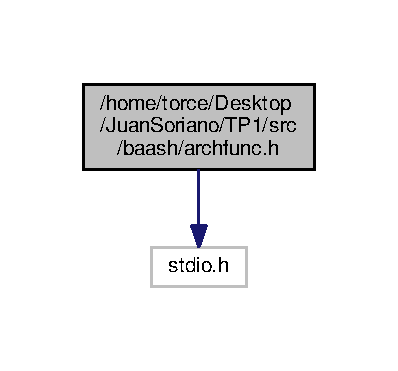
\includegraphics[width=191pt]{archfunc_8h__incl}
\end{center}
\end{figure}
This graph shows which files directly or indirectly include this file\+:
\nopagebreak
\begin{figure}[H]
\begin{center}
\leavevmode
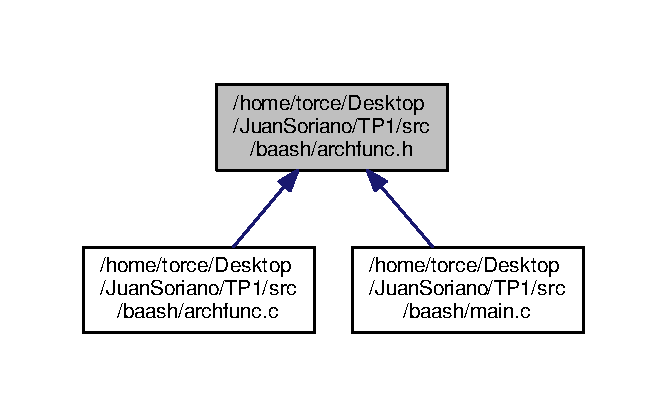
\includegraphics[width=320pt]{archfunc_8h__dep__incl}
\end{center}
\end{figure}
\subsection*{Functions}
\begin{DoxyCompactItemize}
\item 
void {\bf buscar\+Archivo} (char $\ast$file, char $\ast$$\ast$carpetas, char $\ast$command\+File)
\item 
void {\bf a\+Archivo} (char $\ast$archivo)
\item 
void {\bf de\+Archivo} (char filename[$\,$])
\end{DoxyCompactItemize}


\subsection{Function Documentation}
\index{archfunc.\+h@{archfunc.\+h}!a\+Archivo@{a\+Archivo}}
\index{a\+Archivo@{a\+Archivo}!archfunc.\+h@{archfunc.\+h}}
\subsubsection[{a\+Archivo(char $\ast$archivo)}]{\setlength{\rightskip}{0pt plus 5cm}void a\+Archivo (
\begin{DoxyParamCaption}
\item[{char $\ast$}]{archivo}
\end{DoxyParamCaption}
)}\label{archfunc_8h_a1716ae9bb2a53e7f0a27edd9b5ef6b80}
\index{archfunc.\+h@{archfunc.\+h}!buscar\+Archivo@{buscar\+Archivo}}
\index{buscar\+Archivo@{buscar\+Archivo}!archfunc.\+h@{archfunc.\+h}}
\subsubsection[{buscar\+Archivo(char $\ast$file, char $\ast$$\ast$carpetas, char $\ast$command\+File)}]{\setlength{\rightskip}{0pt plus 5cm}void buscar\+Archivo (
\begin{DoxyParamCaption}
\item[{char $\ast$}]{file, }
\item[{char $\ast$$\ast$}]{carpetas, }
\item[{char $\ast$}]{command\+File}
\end{DoxyParamCaption}
)}\label{archfunc_8h_a39bd412666731022a74482418298eab9}
\index{archfunc.\+h@{archfunc.\+h}!de\+Archivo@{de\+Archivo}}
\index{de\+Archivo@{de\+Archivo}!archfunc.\+h@{archfunc.\+h}}
\subsubsection[{de\+Archivo(char filename[])}]{\setlength{\rightskip}{0pt plus 5cm}void de\+Archivo (
\begin{DoxyParamCaption}
\item[{char}]{filename[$\,$]}
\end{DoxyParamCaption}
)}\label{archfunc_8h_abd4ff40c4d09e464acdf313a1be515c5}

\section{/home/torce/\+Desktop/\+Juan\+Soriano/\+T\+P1/src/baash/evalfunc.c File Reference}
\label{evalfunc_8c}\index{/home/torce/\+Desktop/\+Juan\+Soriano/\+T\+P1/src/baash/evalfunc.\+c@{/home/torce/\+Desktop/\+Juan\+Soriano/\+T\+P1/src/baash/evalfunc.\+c}}
{\ttfamily \#include $<$stdio.\+h$>$}\\*
{\ttfamily \#include $<$stdlib.\+h$>$}\\*
{\ttfamily \#include $<$string.\+h$>$}\\*
{\ttfamily \#include \char`\"{}evalfunc.\+h\char`\"{}}\\*
Include dependency graph for evalfunc.\+c\+:
\nopagebreak
\begin{figure}[H]
\begin{center}
\leavevmode
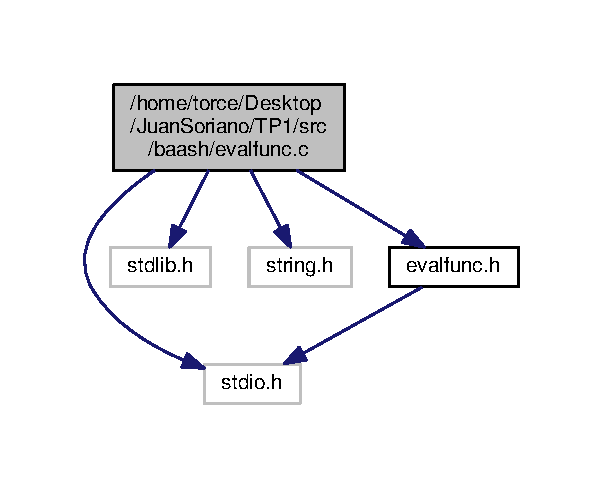
\includegraphics[width=289pt]{evalfunc_8c__incl}
\end{center}
\end{figure}
\subsection*{Functions}
\begin{DoxyCompactItemize}
\item 
int {\bf evaluar\+Pipe} (char $\ast$$\ast$argv, char $\ast$$\ast$argv1, char $\ast$$\ast$argv2)
\item 
int {\bf evaluar\+Background} (char $\ast$$\ast$argv)
\item 
int {\bf evaluar\+Redir} (char $\ast$$\ast$argv, char $\ast$filename)
\end{DoxyCompactItemize}


\subsection{Function Documentation}
\index{evalfunc.\+c@{evalfunc.\+c}!evaluar\+Background@{evaluar\+Background}}
\index{evaluar\+Background@{evaluar\+Background}!evalfunc.\+c@{evalfunc.\+c}}
\subsubsection[{evaluar\+Background(char $\ast$$\ast$argv)}]{\setlength{\rightskip}{0pt plus 5cm}int evaluar\+Background (
\begin{DoxyParamCaption}
\item[{char $\ast$$\ast$}]{argv}
\end{DoxyParamCaption}
)}\label{evalfunc_8c_a3049180ff754a5df764a636dcc595deb}
\index{evalfunc.\+c@{evalfunc.\+c}!evaluar\+Pipe@{evaluar\+Pipe}}
\index{evaluar\+Pipe@{evaluar\+Pipe}!evalfunc.\+c@{evalfunc.\+c}}
\subsubsection[{evaluar\+Pipe(char $\ast$$\ast$argv, char $\ast$$\ast$argv1, char $\ast$$\ast$argv2)}]{\setlength{\rightskip}{0pt plus 5cm}int evaluar\+Pipe (
\begin{DoxyParamCaption}
\item[{char $\ast$$\ast$}]{argv, }
\item[{char $\ast$$\ast$}]{argv1, }
\item[{char $\ast$$\ast$}]{argv2}
\end{DoxyParamCaption}
)}\label{evalfunc_8c_abe29e383eb5f7504acc24f52bd237922}
\index{evalfunc.\+c@{evalfunc.\+c}!evaluar\+Redir@{evaluar\+Redir}}
\index{evaluar\+Redir@{evaluar\+Redir}!evalfunc.\+c@{evalfunc.\+c}}
\subsubsection[{evaluar\+Redir(char $\ast$$\ast$argv, char $\ast$filename)}]{\setlength{\rightskip}{0pt plus 5cm}int evaluar\+Redir (
\begin{DoxyParamCaption}
\item[{char $\ast$$\ast$}]{argv, }
\item[{char $\ast$}]{filename}
\end{DoxyParamCaption}
)}\label{evalfunc_8c_a31a446b63e357548023214ca2320a0a0}

\section{/home/torce/\+Desktop/\+Juan\+Soriano/\+T\+P1/src/baash/evalfunc.h File Reference}
\label{evalfunc_8h}\index{/home/torce/\+Desktop/\+Juan\+Soriano/\+T\+P1/src/baash/evalfunc.\+h@{/home/torce/\+Desktop/\+Juan\+Soriano/\+T\+P1/src/baash/evalfunc.\+h}}
{\ttfamily \#include $<$stdio.\+h$>$}\\*
Include dependency graph for evalfunc.\+h\+:
\nopagebreak
\begin{figure}[H]
\begin{center}
\leavevmode
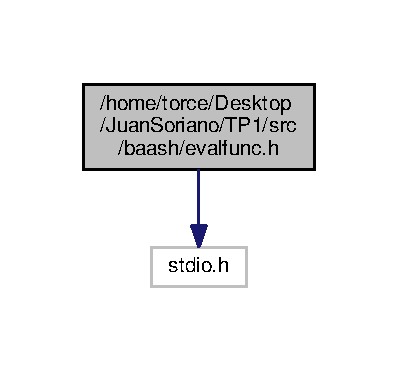
\includegraphics[width=191pt]{evalfunc_8h__incl}
\end{center}
\end{figure}
This graph shows which files directly or indirectly include this file\+:
\nopagebreak
\begin{figure}[H]
\begin{center}
\leavevmode
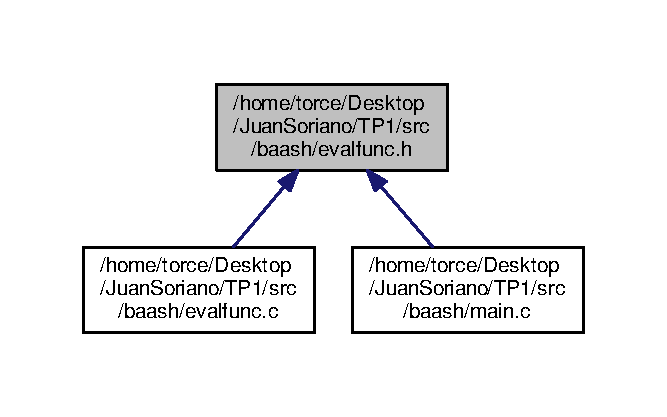
\includegraphics[width=320pt]{evalfunc_8h__dep__incl}
\end{center}
\end{figure}
\subsection*{Functions}
\begin{DoxyCompactItemize}
\item 
int {\bf evaluar\+Pipe} (char $\ast$$\ast$argv, char $\ast$$\ast$argv1, char $\ast$$\ast$argv2)
\item 
int {\bf evaluar\+Background} (char $\ast$$\ast$argv)
\item 
int {\bf evaluar\+Redir} (char $\ast$$\ast$argv, char $\ast$filename)
\end{DoxyCompactItemize}


\subsection{Function Documentation}
\index{evalfunc.\+h@{evalfunc.\+h}!evaluar\+Background@{evaluar\+Background}}
\index{evaluar\+Background@{evaluar\+Background}!evalfunc.\+h@{evalfunc.\+h}}
\subsubsection[{evaluar\+Background(char $\ast$$\ast$argv)}]{\setlength{\rightskip}{0pt plus 5cm}int evaluar\+Background (
\begin{DoxyParamCaption}
\item[{char $\ast$$\ast$}]{argv}
\end{DoxyParamCaption}
)}\label{evalfunc_8h_a3049180ff754a5df764a636dcc595deb}
\index{evalfunc.\+h@{evalfunc.\+h}!evaluar\+Pipe@{evaluar\+Pipe}}
\index{evaluar\+Pipe@{evaluar\+Pipe}!evalfunc.\+h@{evalfunc.\+h}}
\subsubsection[{evaluar\+Pipe(char $\ast$$\ast$argv, char $\ast$$\ast$argv1, char $\ast$$\ast$argv2)}]{\setlength{\rightskip}{0pt plus 5cm}int evaluar\+Pipe (
\begin{DoxyParamCaption}
\item[{char $\ast$$\ast$}]{argv, }
\item[{char $\ast$$\ast$}]{argv1, }
\item[{char $\ast$$\ast$}]{argv2}
\end{DoxyParamCaption}
)}\label{evalfunc_8h_abe29e383eb5f7504acc24f52bd237922}
\index{evalfunc.\+h@{evalfunc.\+h}!evaluar\+Redir@{evaluar\+Redir}}
\index{evaluar\+Redir@{evaluar\+Redir}!evalfunc.\+h@{evalfunc.\+h}}
\subsubsection[{evaluar\+Redir(char $\ast$$\ast$argv, char $\ast$filename)}]{\setlength{\rightskip}{0pt plus 5cm}int evaluar\+Redir (
\begin{DoxyParamCaption}
\item[{char $\ast$$\ast$}]{argv, }
\item[{char $\ast$}]{filename}
\end{DoxyParamCaption}
)}\label{evalfunc_8h_a31a446b63e357548023214ca2320a0a0}

\section{/home/torce/\+Desktop/\+Juan\+Soriano/\+T\+P1/src/baash/main.c File Reference}
\label{baash_2main_8c}\index{/home/torce/\+Desktop/\+Juan\+Soriano/\+T\+P1/src/baash/main.\+c@{/home/torce/\+Desktop/\+Juan\+Soriano/\+T\+P1/src/baash/main.\+c}}
{\ttfamily \#include $<$stdio.\+h$>$}\\*
{\ttfamily \#include $<$stdlib.\+h$>$}\\*
{\ttfamily \#include $<$unistd.\+h$>$}\\*
{\ttfamily \#include $<$pwd.\+h$>$}\\*
{\ttfamily \#include $<$sys/wait.\+h$>$}\\*
{\ttfamily \#include $<$string.\+h$>$}\\*
{\ttfamily \#include \char`\"{}evalfunc.\+h\char`\"{}}\\*
{\ttfamily \#include \char`\"{}archfunc.\+h\char`\"{}}\\*
Include dependency graph for main.\+c\+:
\nopagebreak
\begin{figure}[H]
\begin{center}
\leavevmode
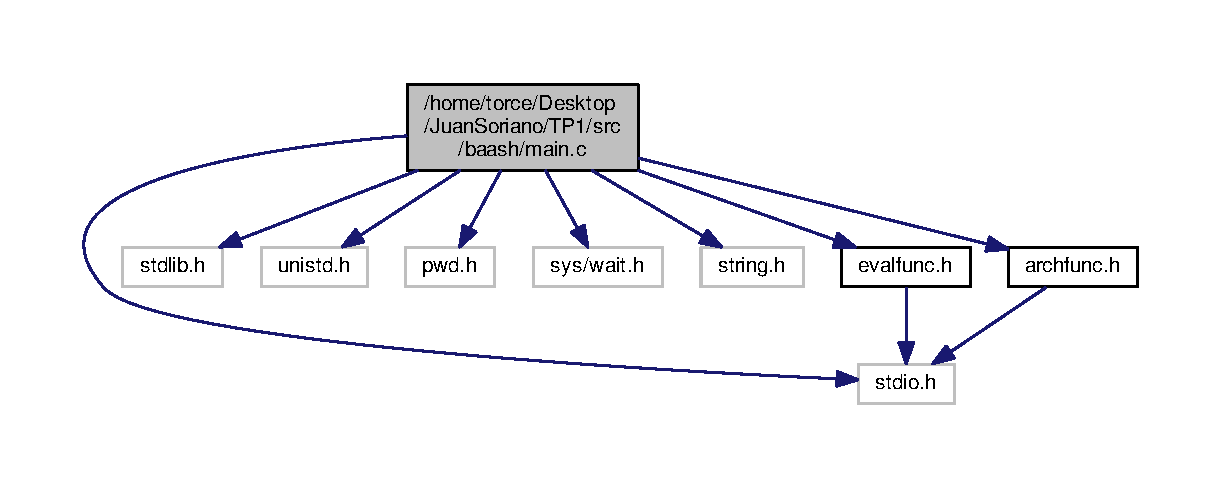
\includegraphics[width=350pt]{baash_2main_8c__incl}
\end{center}
\end{figure}
\subsection*{Functions}
\begin{DoxyCompactItemize}
\item 
void {\bf ejec\+Pipeline} (char $\ast$argv1[$\,$], char $\ast$argv2[$\,$], char $\ast$folders[$\,$])
\item 
int {\bf parsear\+Path} (char $\ast$$\ast$folders)
\item 
int {\bf leer\+Teclado} (char $\ast$$\ast$argv, char $\ast$input)
\item 
int {\bf main} ()
\end{DoxyCompactItemize}


\subsection{Function Documentation}
\index{baash/main.\+c@{baash/main.\+c}!ejec\+Pipeline@{ejec\+Pipeline}}
\index{ejec\+Pipeline@{ejec\+Pipeline}!baash/main.\+c@{baash/main.\+c}}
\subsubsection[{ejec\+Pipeline(char $\ast$argv1[], char $\ast$argv2[], char $\ast$folders[])}]{\setlength{\rightskip}{0pt plus 5cm}void ejec\+Pipeline (
\begin{DoxyParamCaption}
\item[{char $\ast$}]{argv1[$\,$], }
\item[{char $\ast$}]{argv2[$\,$], }
\item[{char $\ast$}]{folders[$\,$]}
\end{DoxyParamCaption}
)}\label{baash_2main_8c_aa274cdfe5fcb3a40ba270054d00a25d3}
\index{baash/main.\+c@{baash/main.\+c}!leer\+Teclado@{leer\+Teclado}}
\index{leer\+Teclado@{leer\+Teclado}!baash/main.\+c@{baash/main.\+c}}
\subsubsection[{leer\+Teclado(char $\ast$$\ast$argv, char $\ast$input)}]{\setlength{\rightskip}{0pt plus 5cm}int leer\+Teclado (
\begin{DoxyParamCaption}
\item[{char $\ast$$\ast$}]{argv, }
\item[{char $\ast$}]{input}
\end{DoxyParamCaption}
)}\label{baash_2main_8c_a6cf44a786e4833cad3ab99ca4e94eb26}
\index{baash/main.\+c@{baash/main.\+c}!main@{main}}
\index{main@{main}!baash/main.\+c@{baash/main.\+c}}
\subsubsection[{main()}]{\setlength{\rightskip}{0pt plus 5cm}int main (
\begin{DoxyParamCaption}
\item[{void}]{}
\end{DoxyParamCaption}
)}\label{baash_2main_8c_ae66f6b31b5ad750f1fe042a706a4e3d4}
\index{baash/main.\+c@{baash/main.\+c}!parsear\+Path@{parsear\+Path}}
\index{parsear\+Path@{parsear\+Path}!baash/main.\+c@{baash/main.\+c}}
\subsubsection[{parsear\+Path(char $\ast$$\ast$folders)}]{\setlength{\rightskip}{0pt plus 5cm}int parsear\+Path (
\begin{DoxyParamCaption}
\item[{char $\ast$$\ast$}]{folders}
\end{DoxyParamCaption}
)}\label{baash_2main_8c_abd7986e5722f366135c2b545c94433de}

\section{/home/torce/\+Desktop/\+Juan\+Soriano/\+T\+P1/src/client/main.c File Reference}
\label{client_2main_8c}\index{/home/torce/\+Desktop/\+Juan\+Soriano/\+T\+P1/src/client/main.\+c@{/home/torce/\+Desktop/\+Juan\+Soriano/\+T\+P1/src/client/main.\+c}}
{\ttfamily \#include $<$arpa/inet.\+h$>$}\\*
{\ttfamily \#include $<$pthread.\+h$>$}\\*
{\ttfamily \#include $<$stdio.\+h$>$}\\*
{\ttfamily \#include $<$stdlib.\+h$>$}\\*
{\ttfamily \#include $<$string.\+h$>$}\\*
Include dependency graph for main.\+c\+:
\nopagebreak
\begin{figure}[H]
\begin{center}
\leavevmode
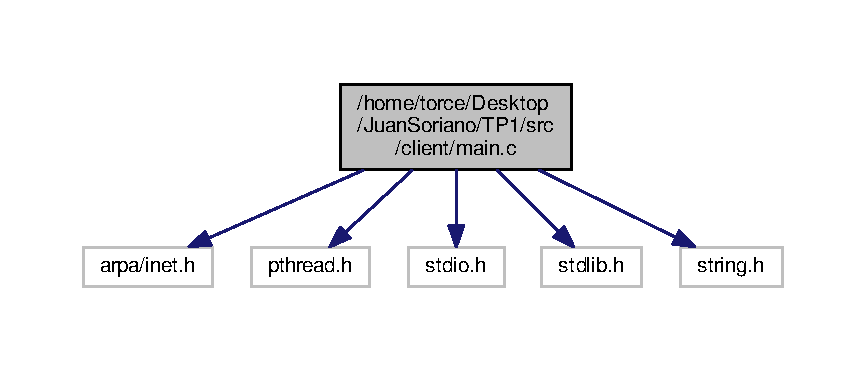
\includegraphics[width=350pt]{client_2main_8c__incl}
\end{center}
\end{figure}
\subsection*{Data Structures}
\begin{DoxyCompactItemize}
\item 
struct {\bf sockbuff}
\end{DoxyCompactItemize}
\subsection*{Macros}
\begin{DoxyCompactItemize}
\item 
\#define {\bf B\+U\+F\+F\+\_\+\+S\+I\+ZE}~1024
\end{DoxyCompactItemize}
\subsection*{Functions}
\begin{DoxyCompactItemize}
\item 
void $\ast$ {\bf writeto\+\_\+socket} (void $\ast$arg)
\item 
int {\bf U\+D\+Pcom} (uint16\+\_\+t U\+D\+Pport, char $\ast${\bf ipaddr}, char $\ast$filename)
\item 
int {\bf main} (void)
\end{DoxyCompactItemize}
\subsection*{Variables}
\begin{DoxyCompactItemize}
\item 
uint16\+\_\+t {\bf portnr}
\item 
char {\bf ipaddrbuff} [20]
\item 
char $\ast$ {\bf ipaddr} = N\+U\+LL
\end{DoxyCompactItemize}


\subsection{Macro Definition Documentation}
\index{client/main.\+c@{client/main.\+c}!B\+U\+F\+F\+\_\+\+S\+I\+ZE@{B\+U\+F\+F\+\_\+\+S\+I\+ZE}}
\index{B\+U\+F\+F\+\_\+\+S\+I\+ZE@{B\+U\+F\+F\+\_\+\+S\+I\+ZE}!client/main.\+c@{client/main.\+c}}
\subsubsection[{B\+U\+F\+F\+\_\+\+S\+I\+ZE}]{\setlength{\rightskip}{0pt plus 5cm}\#define B\+U\+F\+F\+\_\+\+S\+I\+ZE~1024}\label{client_2main_8c_a6c7cd32e1bac137f05e4a752b4ad10af}


\subsection{Function Documentation}
\index{client/main.\+c@{client/main.\+c}!main@{main}}
\index{main@{main}!client/main.\+c@{client/main.\+c}}
\subsubsection[{main(void)}]{\setlength{\rightskip}{0pt plus 5cm}int main (
\begin{DoxyParamCaption}
\item[{void}]{}
\end{DoxyParamCaption}
)}\label{client_2main_8c_a840291bc02cba5474a4cb46a9b9566fe}
\index{client/main.\+c@{client/main.\+c}!U\+D\+Pcom@{U\+D\+Pcom}}
\index{U\+D\+Pcom@{U\+D\+Pcom}!client/main.\+c@{client/main.\+c}}
\subsubsection[{U\+D\+Pcom(uint16\+\_\+t U\+D\+Pport, char $\ast$ipaddr, char $\ast$filename)}]{\setlength{\rightskip}{0pt plus 5cm}int U\+D\+Pcom (
\begin{DoxyParamCaption}
\item[{uint16\+\_\+t}]{U\+D\+Pport, }
\item[{char $\ast$}]{ipaddr, }
\item[{char $\ast$}]{filename}
\end{DoxyParamCaption}
)}\label{client_2main_8c_add2fd8352dfabf670d945c186e88c8e2}
genera una peticion de descarga de un archivo al servidor por socket U\+DP 
\begin{DoxyParams}{Parameters}
{\em U\+D\+Pport} & es el puerto que el servidor le asigno al cliente \\
\hline
{\em ipaddr} & es la direccion ip \\
\hline
{\em filename} & es el nombre del archivo que se quiere descargar\\
\hline
\end{DoxyParams}
\index{client/main.\+c@{client/main.\+c}!writeto\+\_\+socket@{writeto\+\_\+socket}}
\index{writeto\+\_\+socket@{writeto\+\_\+socket}!client/main.\+c@{client/main.\+c}}
\subsubsection[{writeto\+\_\+socket(void $\ast$arg)}]{\setlength{\rightskip}{0pt plus 5cm}void $\ast$ writeto\+\_\+socket (
\begin{DoxyParamCaption}
\item[{void $\ast$}]{arg}
\end{DoxyParamCaption}
)}\label{client_2main_8c_a9d825e493ed30efa51be0621711d2016}
toma los datos ingresados por el teclado y parsea lo ingresado para ver si se trata de un comando o una descarga. 
\begin{DoxyParams}{Parameters}
{\em arg} & es un puntero a la direccion en memoria del struct sockbuff\\
\hline
\end{DoxyParams}


\subsection{Variable Documentation}
\index{client/main.\+c@{client/main.\+c}!ipaddr@{ipaddr}}
\index{ipaddr@{ipaddr}!client/main.\+c@{client/main.\+c}}
\subsubsection[{ipaddr}]{\setlength{\rightskip}{0pt plus 5cm}char$\ast$ ipaddr = N\+U\+LL}\label{client_2main_8c_ad540706412769097e113feb208f0b6bf}
\index{client/main.\+c@{client/main.\+c}!ipaddrbuff@{ipaddrbuff}}
\index{ipaddrbuff@{ipaddrbuff}!client/main.\+c@{client/main.\+c}}
\subsubsection[{ipaddrbuff}]{\setlength{\rightskip}{0pt plus 5cm}char ipaddrbuff[20]}\label{client_2main_8c_a8d57647647f5833d4b1fd30627072575}
\index{client/main.\+c@{client/main.\+c}!portnr@{portnr}}
\index{portnr@{portnr}!client/main.\+c@{client/main.\+c}}
\subsubsection[{portnr}]{\setlength{\rightskip}{0pt plus 5cm}uint16\+\_\+t portnr}\label{client_2main_8c_a10fff5773beb16729c478f6d20e5d986}

\section{/home/torce/\+Facultad/\+S\+O2/so2/\+T\+P1/src/server/main.c File Reference}
\label{server_2main_8c}\index{/home/torce/Facultad/SO2/so2/TP1/src/server/main.c@{/home/torce/Facultad/SO2/so2/TP1/src/server/main.c}}
{\ttfamily \#include $<$netinet/in.\+h$>$}\newline
{\ttfamily \#include $<$stdio.\+h$>$}\newline
{\ttfamily \#include $<$stdlib.\+h$>$}\newline
{\ttfamily \#include $<$string.\+h$>$}\newline
{\ttfamily \#include $<$sys/socket.\+h$>$}\newline
{\ttfamily \#include $<$unistd.\+h$>$}\newline
{\ttfamily \#include $<$signal.\+h$>$}\newline
{\ttfamily \#include $<$arpa/inet.\+h$>$}\newline
{\ttfamily \#include $<$fcntl.\+h$>$}\newline
{\ttfamily \#include $<$sys/stat.\+h$>$}\newline
{\ttfamily \#include $<$pthread.\+h$>$}\newline
{\ttfamily \#include $<$sys/time.\+h$>$}\newline
Include dependency graph for main.\+c\+:
\nopagebreak
\begin{figure}[H]
\begin{center}
\leavevmode
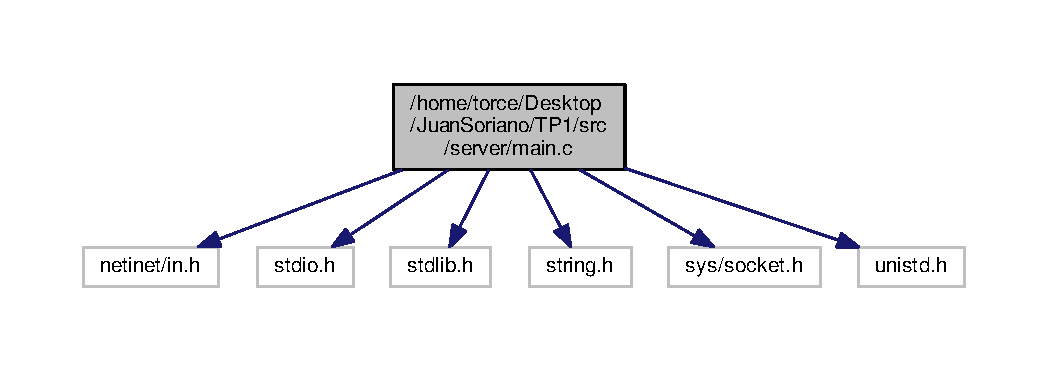
\includegraphics[width=350pt]{server_2main_8c__incl}
\end{center}
\end{figure}
\subsection*{Data Structures}
\begin{DoxyCompactItemize}
\item 
struct \textbf{ Login}
\end{DoxyCompactItemize}
\subsection*{Macros}
\begin{DoxyCompactItemize}
\item 
\#define \textbf{ L\+I\+S\+T\+E\+N\+\_\+\+P\+O\+RT}~2019
\item 
\#define \textbf{ U\+D\+P\+\_\+\+C\+L\+I\+E\+N\+T\+\_\+\+P\+O\+RT}~2019
\item 
\#define \textbf{ S\+N\+A\+ME}~20
\item 
\#define \textbf{ U\+S\+E\+R\+\_\+\+NR}~2
\item 
\#define \textbf{ B\+U\+F\+F\+\_\+\+S\+I\+ZE}~1024
\item 
\#define \textbf{ F\+I\+L\+E\+\_\+\+B\+U\+F\+F\+E\+R\+\_\+\+S\+I\+ZE}~1500
\item 
\#define \textbf{ R\+E\+T\+R\+Y\+\_\+\+L\+I\+M\+IT}~3
\item 
\#define \textbf{ F\+I\+R\+M\+W\+A\+R\+E\+\_\+\+F\+I\+LE}~\char`\"{}../updated\+\_\+client\char`\"{}
\item 
\#define \textbf{ I\+M\+A\+G\+E\+\_\+\+F\+I\+LE}~\char`\"{}../incoming\+\_\+2019.\+jpg\char`\"{}
\end{DoxyCompactItemize}
\subsection*{Functions}
\begin{DoxyCompactItemize}
\item 
int \textbf{ verificar} (char $\ast$user, char $\ast$password)
\begin{DoxyCompactList}\small\item\em Verifica del lado del server que los datos ingresados por el cliente correspondan a un usuario registrado. \end{DoxyCompactList}\item 
int \textbf{ get\+Telemetria} (char $\ast$\textbf{ ipaddr})
\begin{DoxyCompactList}\small\item\em Abre un socket U\+DP para recibir la telemetria del satelite y la muestra por pantalla. \end{DoxyCompactList}\item 
int \textbf{ get\+Scan} (int sockfd2)
\begin{DoxyCompactList}\small\item\em Obtiene la imagen (scan) del satelite por medio del socket T\+CP ya instanciado. \end{DoxyCompactList}\item 
int \textbf{ send\+Update} (int sockfd)
\begin{DoxyCompactList}\small\item\em Envia un update de firmware a los satelites que se encuentran escuchando por medio de T\+CP. \end{DoxyCompactList}\item 
int \textbf{ main} (void)
\begin{DoxyCompactList}\small\item\em Servidor que simula base terrestre. \end{DoxyCompactList}\end{DoxyCompactItemize}


\subsection{Macro Definition Documentation}
\mbox{\label{server_2main_8c_a6c7cd32e1bac137f05e4a752b4ad10af}} 
\index{main.c@{main.c}!BUFF\_SIZE@{BUFF\_SIZE}}
\index{BUFF\_SIZE@{BUFF\_SIZE}!main.c@{main.c}}
\subsubsection{BUFF\_SIZE}
{\footnotesize\ttfamily \#define B\+U\+F\+F\+\_\+\+S\+I\+ZE~1024}

\mbox{\label{server_2main_8c_a09dbbd73a84cf772b421c6024b65b1fd}} 
\index{main.c@{main.c}!FILE\_BUFFER\_SIZE@{FILE\_BUFFER\_SIZE}}
\index{FILE\_BUFFER\_SIZE@{FILE\_BUFFER\_SIZE}!main.c@{main.c}}
\subsubsection{FILE\_BUFFER\_SIZE}
{\footnotesize\ttfamily \#define F\+I\+L\+E\+\_\+\+B\+U\+F\+F\+E\+R\+\_\+\+S\+I\+ZE~1500}

\mbox{\label{server_2main_8c_a6ef7baa1d4325116155fe508770ec911}} 
\index{main.c@{main.c}!FIRMWARE\_FILE@{FIRMWARE\_FILE}}
\index{FIRMWARE\_FILE@{FIRMWARE\_FILE}!main.c@{main.c}}
\subsubsection{FIRMWARE\_FILE}
{\footnotesize\ttfamily \#define F\+I\+R\+M\+W\+A\+R\+E\+\_\+\+F\+I\+LE~\char`\"{}../updated\+\_\+client\char`\"{}}

\mbox{\label{server_2main_8c_ade64ea695c038c15864c1e6fd5d69c03}} 
\index{main.c@{main.c}!IMAGE\_FILE@{IMAGE\_FILE}}
\index{IMAGE\_FILE@{IMAGE\_FILE}!main.c@{main.c}}
\subsubsection{IMAGE\_FILE}
{\footnotesize\ttfamily \#define I\+M\+A\+G\+E\+\_\+\+F\+I\+LE~\char`\"{}../incoming\+\_\+2019.\+jpg\char`\"{}}

\mbox{\label{server_2main_8c_a4fba0963c20988d1f1a45afb1c636e44}} 
\index{main.c@{main.c}!LISTEN\_PORT@{LISTEN\_PORT}}
\index{LISTEN\_PORT@{LISTEN\_PORT}!main.c@{main.c}}
\subsubsection{LISTEN\_PORT}
{\footnotesize\ttfamily \#define L\+I\+S\+T\+E\+N\+\_\+\+P\+O\+RT~2019}

\mbox{\label{server_2main_8c_ad4eba3b0ea03f397bae8792d0f0e4cd4}} 
\index{main.c@{main.c}!RETRY\_LIMIT@{RETRY\_LIMIT}}
\index{RETRY\_LIMIT@{RETRY\_LIMIT}!main.c@{main.c}}
\subsubsection{RETRY\_LIMIT}
{\footnotesize\ttfamily \#define R\+E\+T\+R\+Y\+\_\+\+L\+I\+M\+IT~3}

\mbox{\label{server_2main_8c_adbe6c60fb689b6eb1c165dda1b4ccda1}} 
\index{main.c@{main.c}!SNAME@{SNAME}}
\index{SNAME@{SNAME}!main.c@{main.c}}
\subsubsection{SNAME}
{\footnotesize\ttfamily \#define S\+N\+A\+ME~20}

\mbox{\label{server_2main_8c_a3875beebc35d95ef6312fc484bf5adac}} 
\index{main.c@{main.c}!UDP\_CLIENT\_PORT@{UDP\_CLIENT\_PORT}}
\index{UDP\_CLIENT\_PORT@{UDP\_CLIENT\_PORT}!main.c@{main.c}}
\subsubsection{UDP\_CLIENT\_PORT}
{\footnotesize\ttfamily \#define U\+D\+P\+\_\+\+C\+L\+I\+E\+N\+T\+\_\+\+P\+O\+RT~2019}

\mbox{\label{server_2main_8c_ad5b70b0fae15f71d75dfd3110e8ff522}} 
\index{main.c@{main.c}!USER\_NR@{USER\_NR}}
\index{USER\_NR@{USER\_NR}!main.c@{main.c}}
\subsubsection{USER\_NR}
{\footnotesize\ttfamily \#define U\+S\+E\+R\+\_\+\+NR~2}



\subsection{Function Documentation}
\mbox{\label{server_2main_8c_ad0fd16b59ec0ac5a66429c8dad254b8e}} 
\index{main.c@{main.c}!getScan@{getScan}}
\index{getScan@{getScan}!main.c@{main.c}}
\subsubsection{getScan()}
{\footnotesize\ttfamily int get\+Scan (\begin{DoxyParamCaption}\item[{int}]{sockfd2 }\end{DoxyParamCaption})}



Obtiene la imagen (scan) del satelite por medio del socket T\+CP ya instanciado. 


\begin{DoxyParams}{Parameters}
{\em sockfd2} & file descriptor del socket T\+CP abierto para la recepcion de la imagen \\
\hline
\end{DoxyParams}
\begin{DoxyReturn}{Returns}
int 0\+: no se pudo abrir el archivo para escritura. int 1\+: se termino la recepcion exitosamente. 
\end{DoxyReturn}
\mbox{\label{server_2main_8c_ad7764287b17ffb0a84baf8a23275edec}} 
\index{main.c@{main.c}!getTelemetria@{getTelemetria}}
\index{getTelemetria@{getTelemetria}!main.c@{main.c}}
\subsubsection{getTelemetria()}
{\footnotesize\ttfamily int get\+Telemetria (\begin{DoxyParamCaption}\item[{char $\ast$}]{ipaddr }\end{DoxyParamCaption})}



Abre un socket U\+DP para recibir la telemetria del satelite y la muestra por pantalla. 


\begin{DoxyParams}{Parameters}
{\em ipaddr} & direccion ip del satelite conectado proveniente de la estructura almacenada de la conexion tcp \\
\hline
\end{DoxyParams}
\begin{DoxyReturn}{Returns}
int 1\+: recepcion exitosa (no asegura que la informacion sea valida). int 0\+: error en la conexion. 
\end{DoxyReturn}
\mbox{\label{server_2main_8c_a840291bc02cba5474a4cb46a9b9566fe}} 
\index{main.c@{main.c}!main@{main}}
\index{main@{main}!main.c@{main.c}}
\subsubsection{main()}
{\footnotesize\ttfamily int main (\begin{DoxyParamCaption}\item[{void}]{ }\end{DoxyParamCaption})}



Servidor que simula base terrestre. 

Se realiza una etapa de autenticacion por parte del usuario en la base de datos del servidor. Si se acepta, Se continua y se acepta conexiones con los satelites. Se ofrece un prompt para ingresar comandos. \mbox{\label{server_2main_8c_a399ed36a71efbd160709be4b09406574}} 
\index{main.c@{main.c}!sendUpdate@{sendUpdate}}
\index{sendUpdate@{sendUpdate}!main.c@{main.c}}
\subsubsection{sendUpdate()}
{\footnotesize\ttfamily int send\+Update (\begin{DoxyParamCaption}\item[{int}]{sockfd }\end{DoxyParamCaption})}



Envia un update de firmware a los satelites que se encuentran escuchando por medio de T\+CP. 


\begin{DoxyParams}{Parameters}
{\em sockfd} & File descriptor del socket abierto T\+CP. \\
\hline
\end{DoxyParams}
\begin{DoxyReturn}{Returns}
int 1\+: envio exitoso. int 0\+: hubo un error en la apertura del archivo para enviar. 
\end{DoxyReturn}
\mbox{\label{server_2main_8c_a8ebfa03aaa653d8fc17a3d498a22cb40}} 
\index{main.c@{main.c}!verificar@{verificar}}
\index{verificar@{verificar}!main.c@{main.c}}
\subsubsection{verificar()}
{\footnotesize\ttfamily int verificar (\begin{DoxyParamCaption}\item[{char $\ast$}]{user,  }\item[{char $\ast$}]{password }\end{DoxyParamCaption})}



Verifica del lado del server que los datos ingresados por el cliente correspondan a un usuario registrado. 


\begin{DoxyParams}{Parameters}
{\em user} & el nombre de usuario ingresado \\
\hline
{\em password} & el password ingresado \\
\hline
\end{DoxyParams}
\begin{DoxyReturn}{Returns}
int 0\+: no autenticado, 1\+:autenticado. 
\end{DoxyReturn}

%--- End generated contents ---

% Index
\backmatter
\newpage
\phantomsection
\clearemptydoublepage
\addcontentsline{toc}{chapter}{Index}
\printindex

\end{document}
